\documentclass[a4paper,12pt]{report}
\usepackage[utf8]{inputenc}
\usepackage{graphicx}
\usepackage{hyperref}

\begin{document}

% Title Page
\begin{titlepage}
    \centering
    \vspace*{1.5cm}
    
    {\Huge \textbf{Smart office preferences manager}} \\[1.5cm]
    
    {\Large \textbf{PRIOT Project}} \\[2.5cm]
    
    \textbf{Author:} \\[0.5cm]
    {\Large Dragomir Andrei-Mihai 343C1} \\[2.5cm]
    
    \textbf{Description:} \\[0.5cm]
    \parbox{0.8\textwidth}{
        Documentation for the design and implementation of a smart in office logger,
        an IoT system for managing employee access and monitoring environmental conditions. The system integrates hardware components such as RFID, sensors, and an ESP32 microcontroller, and communicates with a server for centralized data visualization and management.
    }
    
    \vfill
    {\Large \textbf{\today}} \\[1.5cm]
\end{titlepage}

% Table of Contents Page
\newpage
\tableofcontents
\newpage

% Chapters Start
\chapter{Introduction}

This paper describes the implementation of an IoT system for managing employee access and monitoring the environment in the office (temperature and humidity). The project combines a sensor network with an ESP32 hub that communicates with a central server to store and visualize data.

Employees receive alerts when the temperature or humidity is not optimal for their inputted preferences. The system also logs access events, allowing administrators to monitor employee activity: logins, logouts, access attempts, time spent in the office, etc.

\section{Key Objectives}
\begin{itemize}
    \item Manage employee access through an RFID system.
    \item Monitor the environment using a DHT11 sensor.
    \item Visualize collected data via an interactive web interface.
\end{itemize}

% Architecture Chapter
\chapter{Architecture}

\section{Overview}
This project architecture is designed to achieve modularity and scalability by separating the ESP32 microcontroller logic from the backend server and frontend interface. It uses a combination of hardware, communication protocols, and software layers to deliver the functionality.

\subsection{Backend (Flask Server)}
The backend is implemented using Python and Flask. It serves as the central hub for processing data received from the ESP32, managing user preferences, and rendering the web-based interface for administrators and employees. Key components include:
\begin{itemize}
    \item \textbf{server.py}: The Flask application that handles HTTP requests and serves dynamic HTML pages.
    \item \textbf{templates/}: Contains HTML files used by Flask for dynamic content rendering (e.g., \texttt{preferences.html}, \texttt{records.html}).
    \item \textbf{static/}: Stores frontend assets such as:
        \begin{itemize}
            \item \textbf{CSS}: Styling for the interface (e.g., \texttt{style.css}).
            \item \textbf{JavaScript}: Frontend logic and interactivity (e.g., \texttt{script.js}).
        \end{itemize}
    \item \textbf{users.json}: A lightweight storage file for user data and preferences.
\end{itemize}

\subsection{ESP32 Firmware (C++)}
The ESP32 firmware is written in written in C++. This firmware handles the hardware peripherals and communicates with the Flask server and is organized into several files within the \texttt{src/} directory:
\begin{itemize} 
    \item \textbf{main.cpp}: The entry point for the ESP32 firmware, initializing all components and managing the main logic loop.
    \item \textbf{access\_utils.cpp}: Handles RFID-based access control and logs employee activities such as logins and logouts.
    \item \textbf{http\_utils.cpp}: Manages HTTP communication between the ESP32 and the Flask server for data exchange.
    \item \textbf{led\_buzz\_utils.cpp}: Controls visual and auditory feedback through RGB LEDs and a buzzer.
    \item \textbf{temp\_utils.cpp}: Captures and processes temperature and humidity data using the DHT11 sensor.
    \item \textbf{rtc\_utils.cpp}: Provides accurate timestamps using the RTC module.
    \item \textbf{print\_utils.cpp} and \textbf{utils.hpp}: Utility functions for logging, debugging, and reusability.
\end{itemize}

\newpage

\section{Hardware and Network Schema}
The system uses an ESP32 microcontroller to interact with peripherals and communicate with the backend server over Wi-Fi. The topology is represented as follows:

\begin{figure}[h]
    \centering
    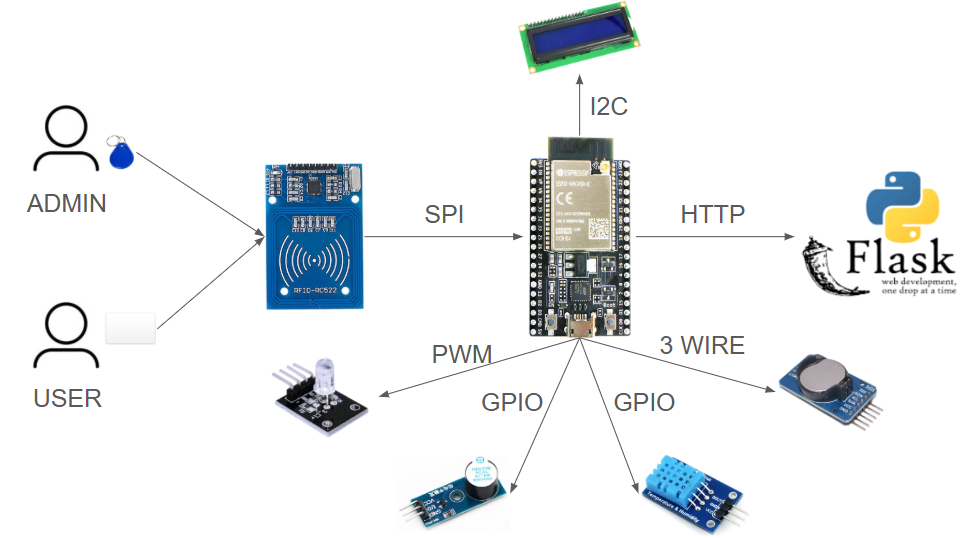
\includegraphics[width=1\textwidth]{img/schema.png}
    \caption{Hardware Schema}
\end{figure}

\subsection{Hardware and Protocols}

The system is designed to integrate various hardware components with the ESP32 microcontroller, which serves as the central hub for communication and control. The following describes the key components and their connections:

\begin{itemize}
    \item \textbf{RFID Reader (SPI Protocol):} The RFID module communicates with the ESP32 using the high-speed SPI protocol. It is used for user authentication and access control. Admins and users interact with the system by scanning their RFID tags or cards.

    \item \textbf{LCD Screen (I2C Protocol):} The LCD display is connected to the ESP32 via the I2C protocol. It provides a user interface for displaying system status, access logs, and environmental data locally.

    \item \textbf{Flask Server (HTTP over Wi-Fi):} The ESP32 communicates with the Flask server using the HTTP protocol over Wi-Fi. This connection is used to send collected data (e.g., RFID access logs and environmental readings) and receive configurations or updates from the server.

    \item \textbf{RGB LED (PWM):} The RGB LED is connected to the ESP32 through GPIO pins configured for PWM (Pulse Width Modulation). It provides visual feedback for operations such as successful logins, errors, or status updates.

    \item \textbf{Buzzer (GPIO):} The buzzer is directly connected to a GPIO pin on the ESP32. It provides auditory feedback for system events, such as login success, login failure, or alerts.

    \item \textbf{DHT11 Sensor (GPIO):} The DHT11 sensor is linked to the ESP32 through a GPIO pin. It captures environmental data, specifically temperature and humidity, which is logged during user interactions.

    \item \textbf{RTC Module (Three-Wire Protocol):} The Real-Time Clock (RTC) module connects to the ESP32 using a three-wire protocol, providing accurate timestamps for logging access events and environmental data.

\end{itemize}

This hardware configuration ensures good communication and reliable data exchange between the various components, with the ESP32 acting as the central coordinator.

\chapter{Implementation}

This system is implemented using a combination of C++ for the ESP32 firmware and Python for the Flask server. The following sections detail the key components and their functionalities.

\section{ESP32 Firmware}

\section{Introduction}
The ESP32 firmware is designed to manage user access, handle environmental data, and provide feedback through LEDs and an LCD display. It also implements secure communication with a Flask server using encrypted requests and responses. This document describes the implementation structure and details for the firmware.

\section{Project Structure}
The firmware is organized into the following files:

\begin{itemize}
    \item \textbf{main.cpp}: Entry point of the firmware.
    \item \textbf{access\_utils.cpp}: Handles user access-related functionalities.
    \item \textbf{http\_utils.cpp}: Manages HTTP requests and server interactions.
    \item \textbf{encryption.cpp}: Implements AES encryption and decryption.
    \item \textbf{led\_buzz\_utils.cpp}: Controls LED and buzzer behaviors.
    \item \textbf{print\_utils.cpp}: Handles LCD printing.
    \item \textbf{rtc\_utils.cpp}: Real-time clock management.
    \item \textbf{temp\_utils.cpp}: Reads and processes temperature and humidity data.
    \item \textbf{utils.cpp, utils.hpp}: Core utilities and global declarations.
\end{itemize}

\section{Hardware Configuration}
\subsection{Pin Assignments}
\begin{itemize}
    \item \textbf{LEDs}: RED\_PIN (17), GREEN\_PIN (4), BLUE\_PIN (2)
    \item \textbf{Buzzer}: BUZZER\_PIN (5)
    \item \textbf{Joystick}: SW\_PIN (34), URX\_PIN (32), URY\_PIN (35)
    \item \textbf{RTC}: CLK\_PIN (33), DAT\_PIN (16), RST\_PIN (15)
    \item \textbf{LCD}: SDA\_PIN (25), SCL\_PIN (26)
    \item \textbf{DHT Sensor}: DHTPIN (13)
\end{itemize}

\subsection{Peripherals}
The following peripherals are utilized:
\begin{itemize}
    \item RFID Module (MFRC522)
    \item LCD Display (LiquidCrystal\_I2C)
    \item Real-Time Clock (DS1302)
    \item DHT11 Temperature and Humidity Sensor
\end{itemize}

\section{Core Functionalities}
\subsection{User Access Management}
\begin{itemize}
    \item \textbf{Add Access}: Allows new users to gain access by storing their UID.
    \item \textbf{Remove Access}: Revokes access for specific users.
    \item \textbf{Authorization}: Checks if a UID is authorized for access.
    \item Functions:
    \begin{itemize}
        \item \texttt{void addCardAccess()}
        \item \texttt{void removeCardAccess()}
        \item \texttt{bool isAuthorizedUID(String uid)}
    \end{itemize}
\end{itemize}

\subsection{Temperature and Humidity Monitoring}
\begin{itemize}
    \item Reads data from the DHT11 sensor.
    \item Provides real-time feedback on the LCD display.
    \item Functions:
    \begin{itemize}
        \item \texttt{void get\_temperature\_humidity(float \&temperature, float \&humidity)}
        \item \texttt{void print\_temperature\_humidity(float temperature, float humidity)}
    \end{itemize}
\end{itemize}

\subsection{Real-Time Clock Management}
\begin{itemize}
    \item Synchronizes and reads date/time.
    \item Converts date/time to integer format for calculations.
    \item Functions:
    \begin{itemize}
        \item \texttt{RtcDateTime readQuartzTime()}
        \item \texttt{void setDateTime()}
    \end{itemize}
\end{itemize}

\subsection{LED and Buzzer Feedback}
\begin{itemize}
    \item Provides visual and audio feedback based on events.
    \item Functions:
    \begin{itemize}
        \item \texttt{void turnOffLEDs()}
        \item \texttt{void goodbyeMelody()}
        \item \texttt{void accessGrantedMelody()}
        \item \texttt{void accessDeniedMelody()}
    \end{itemize}
\end{itemize}

\subsection{HTTP and HTTPS Communication}
\begin{itemize}
    \item Communicates with the Flask server using HTTPS.
    \item Functions:
    \begin{itemize}
        \item \texttt{void sendEmployeeData(String name, String uid, String time, float temperature, float humidity, String reminder, bool inOut)}
        \item \texttt{void fetchUserPreferences(String uid, float \&temperature, float \&humidity)}
    \end{itemize}
\end{itemize}

\section{Alerts and Notification System}

The alerts in this implementation are designed to ensure that users and administrators
are promptly informed about important events and status updates within the platform. 

\subsection{System Overview}
The alerts and notification system monitors key events, such as unauthorized access attempts and changes in user preferences.
Upon detecting such events, the system generates alerts that are sent to the ESP32 board.

\subsection{Implementation on ESP32}
The ESP32 firmware includes functions to trigger audible and visual alerts using LEDs and buzzers. For example:
\begin{itemize}
    \item \textbf{LED Notifications}: RGB LEDs are programmed to display specific colors based on event types (e.g., red for errors, green for successful operations, and blue for general notifications).
    \item \textbf{Audible Alerts}: The buzzer emits predefined melodies or tones to indicate critical alerts, such as unauthorized card access or temperature anomalies.
\end{itemize}

Additionally, the ESP32 sends encrypted notification payloads to the Flask server for centralized logging and processing.

\section{LCD Display Management}
\begin{itemize}
    \item Displays messages and feedback on the LCD.
    \item Functions:
    \begin{itemize}
        \item \texttt{void printStringOnLCD(const char *message)}
        \item \texttt{void showSettingPreferences(float currentTemp, float currentHumid, float preferedTemp, float preferedHumid)}
    \end{itemize}
\end{itemize}

\section{Main Entry Point}
\begin{itemize}
    \item Initializes peripherals, connects to WiFi, and starts the HTTP server.
    \item Functions:
    \begin{itemize}
        \item \texttt{void connectToWiFi()}
        \item \texttt{void setupLEDControl()}
    \end{itemize}
\end{itemize}

\chapter{Visualization and Data Processing}

The Flask server provides visualization and data processing functionalities, offering insights into employee activities, preferences, and environmental conditions. The implementation is structured to process and visualize data dynamically based on the logs and user data.

\section{Data Sources}
The server processes data from two primary sources:
\begin{itemize}
    \item \textbf{User Data}: Loaded from \texttt{users.json}, containing user preferences and access information.
    \item \textbf{Logs}: Stored in \texttt{mock\_logs.json}, tracking employee login/logout activities along with timestamps and environmental conditions.
\end{itemize}

\section{Visualization Dashboard}
The visualization dashboard displays various graphs and statistics, accessible through the \texttt{/visualization} route. Key components include:
\begin{itemize}
    \item \textbf{User Preferences Chart}: Bar graph showing temperature and humidity preferences for each user.
    \item \textbf{Time Series Data}: Line graphs of temperature and humidity over time.
    \item \textbf{All Hours Graph}: Line graph showing the frequency of entries across different hours of the day.
    \item \textbf{Top Visitors}: Bar graph of the most frequent visitors based on logs.
\end{itemize}

The data is processed using Python's \texttt{Counter} and rendered dynamically using Chart.js.

\begin{figure}[h]
    \centering
    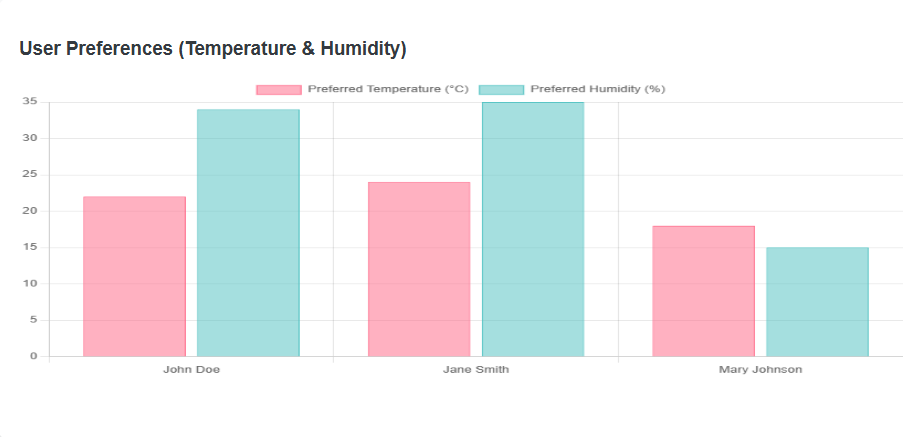
\includegraphics[width=1\textwidth]{img/PreferencesGraph.png}
    \caption{User Preferences Temperature \& Humidity}
\end{figure}

\begin{figure}[h]
    \centering
    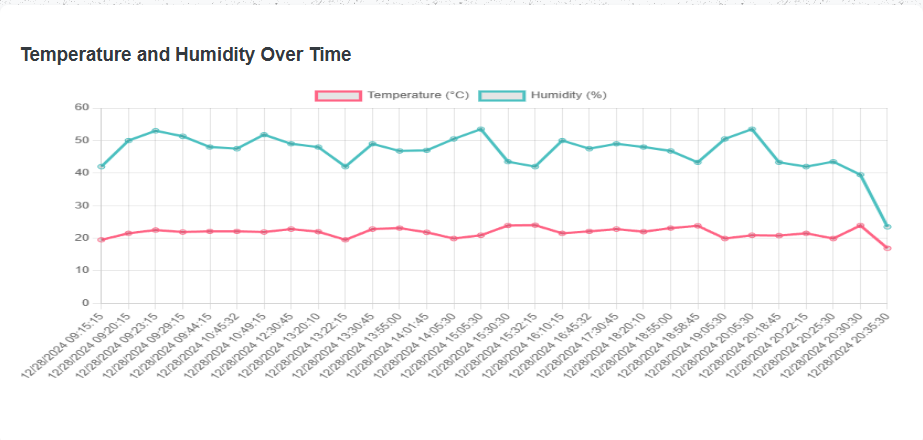
\includegraphics[width=1\textwidth]{img/TempEvolution.png}
    \caption{Temperature and Humidity Over Time}
\end{figure}

\newpage

\begin{figure}[h]
    \centering
    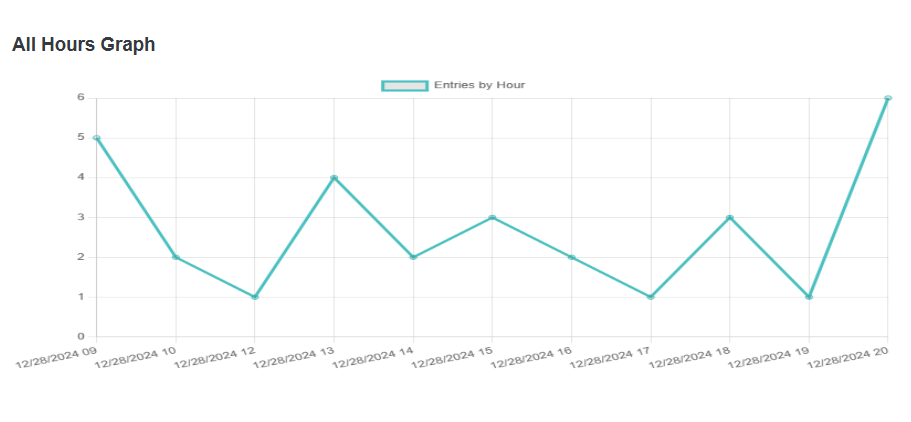
\includegraphics[width=1\textwidth]{img/AllHoursGraph.png}
    \caption{All Hours Graph}
\end{figure}

\begin{figure}[h]
    \centering
    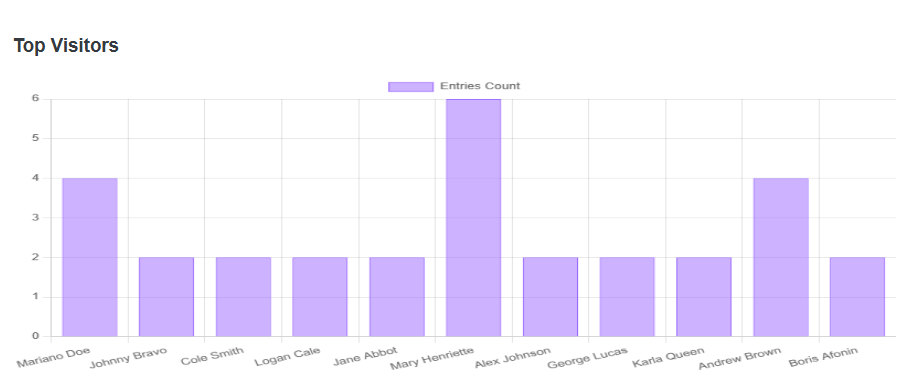
\includegraphics[width=1\textwidth]{img/TopVisitors.png}
    \caption{Top Visitors}
\end{figure}

\newpage

\section{Records Display}
The \texttt{/records} route lists all employee activities in a tabular format:
\begin{itemize}
    \item Name, UID, timestamp, temperature, humidity, reminder, and activity type (login/logout) are shown.
\end{itemize}

\begin{figure}[h]
    \centering
    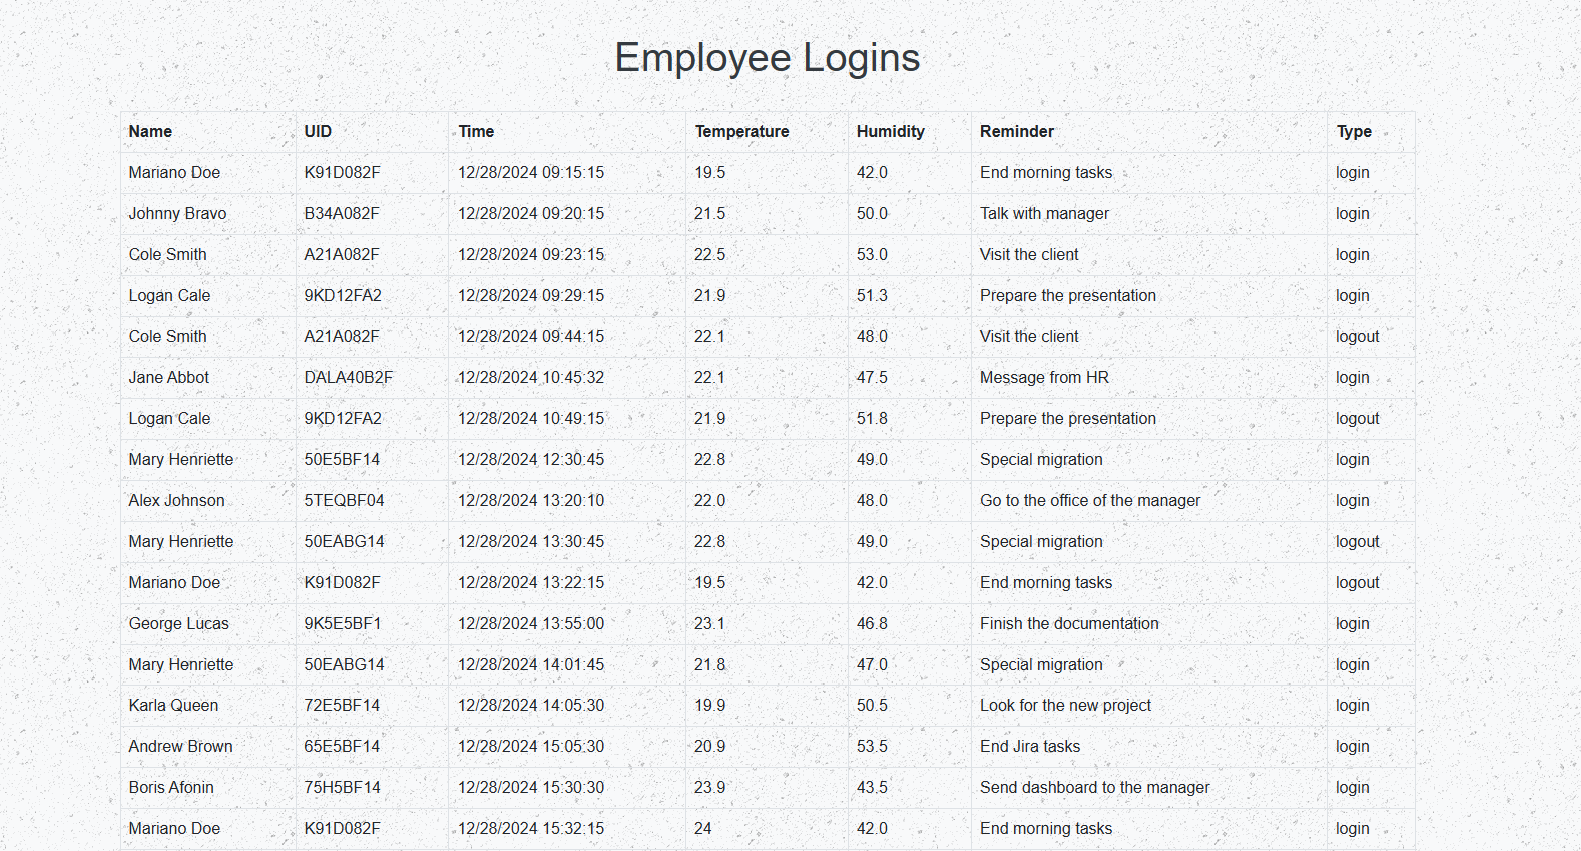
\includegraphics[width=1\textwidth]{img/Records.png}
    \caption{Records Display}
\end{figure}


\begin{figure}[h]
    \centering
    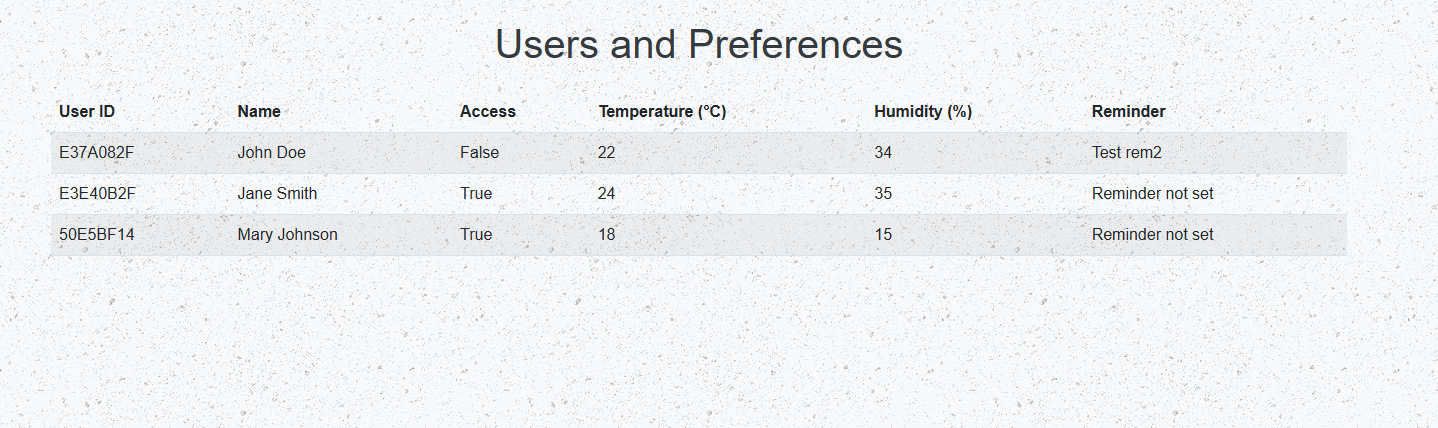
\includegraphics[width=1\textwidth]{img/Users.png}
    \caption{Registered Users Display}
\end{figure}

\begin{figure}[h]
    \centering
    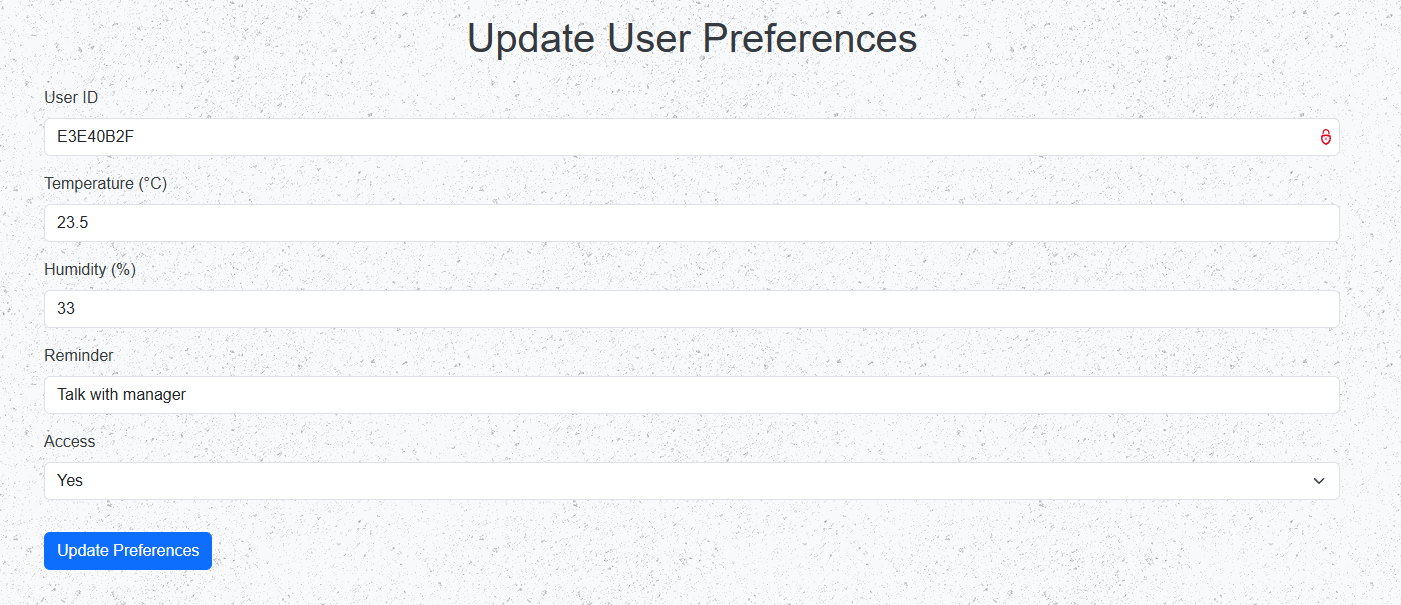
\includegraphics[width=1\textwidth]{img/Update.png}
    \caption{Preferences and Access Update Functionality}
\end{figure}

\section{Data Processing and Analysis}
\subsubsection{Time-Based Sorting}
Employee logs are sorted based on their timestamps for chronological visualization:
\begin{verbatim}
sorted_logs = sorted(logs, key=lambda log: 
    datetime.strptime(log['time'], "%m/%d/%Y %H:%M:%S"))
\end{verbatim}

\subsection{Statistical Aggregation}
Various aggregations are performed using Python's \texttt{Counter}:
\begin{itemize}
    \item Crowded times are derived from timestamps split by hours.
    \item Top visitors are determined based on the frequency of names in logs.
\end{itemize}

\section{Integration with Frontend}
The visualization and records pages are rendered dynamically:
\begin{itemize}
    \item \textbf{HTML Templates}: Templates include Bootstrap for styling and Chart.js for visualizations.
    \item \textbf{Dynamic Rendering}: Data from Flask backend is injected into templates using Jinja2, allowing real-time updates.
\end{itemize}

\section{User Preferences}

The Flask server provides functionalities to manage and update user preferences through the \texttt{/preferences} route. This section allows users to:
\begin{itemize}
    \item View and update individual preferences such as temperature, humidity, and reminders.
    \item Enable or disable access permissions for specific users.
    \item Dynamically fetch and modify preferences via the \texttt{update\_preferences} API.
\end{itemize}

The preferences are stored in \texttt{users.json} and encrypted for secure communication with ESP32 devices. Updates are reflected on the ESP32 firmware in real time.

\section{Alerts}

The system implements an alert mechanism to notify users and employees of specific conditions:
\begin{itemize}
    \item Alerts consist on update for access or preferences for users which directly show up on ESP32 with a led and buzzer notification, as well as LCD display information.
    \item Alerts are communicated securely using encrypted messages to ensure data integrity and confidentiality.
\end{itemize}

\chapter{Security}

\section{Access Control}

The system implements robust access control mechanisms to manage user permissions effectively:
\begin{itemize}
    \item Each user is identified by a unique UID, stored securely in the \texttt{users.json} file.
    \item Access permissions are managed through APIs such as \texttt{/set\_access}, \texttt{/add\_access}, and \texttt{/remove\_access}.
    \item The ESP32 firmware validates UIDs locally to ensure only authorized users can interact with the system.
    \item Administrative privileges are granted based on predefined UIDs, such as \texttt{ADMIN\_UID}, to restrict critical actions like resetting the system or modifying global settings.
\end{itemize}

\section{Protocols}

The system uses secure communication protocols to ensure data integrity and confidentiality:
\begin{itemize}
    \item HTTPS is used for all communications between the ESP32 and the Flask server to protect against man-in-the-middle attacks.
    \item The Flask server utilizes a self-signed SSL certificate, ensuring encrypted data exchange.
    \item The ESP32 employs the WiFiClientSecure library for secure HTTPS requests, supporting modern encryption standards.
    \item The MQTT protocol can be integrated for real-time notifications, employing TLS for secure messaging.
\end{itemize}

\section{Data Encryption}

Data security is enforced through AES-128 encryption:
\begin{itemize}
    \item All sensitive data exchanged between the ESP32 and the Flask server is encrypted using the AES-128 CBC mode.
    \item A pre-shared key (\texttt{aes\_key}) and an initialization vector (\texttt{iv}) are used for encryption and decryption.
    \item The system employs PKCS7 padding to ensure plaintext aligns with the block size required by AES.
    \item Encrypted data is Base64-encoded for compatibility with JSON and HTTP payloads.
    \item Decryption is performed on the receiving end to reconstruct the original data, ensuring end-to-end security.
\end{itemize}

\chapter{Challenges and Solutions}

\section{Challenges}

The development and deployment of the ESP32-based IoT system presented several challenges:

\subsection{Secure Communication}
Implementing secure communication between the ESP32 and the Flask server required careful management of encryption keys and SSL certificates. Debugging encrypted data transmission added complexity due to potential mismatches in encoding and padding.

\subsection{Resource Constraints}
The ESP32's limited memory and processing power posed challenges in handling encryption, parsing large JSON payloads, and managing multiple peripherals concurrently.

\subsection{Data Synchronization}
Ensuring real-time synchronization of user preferences and logs between the server and the ESP32 was challenging, especially during network interruptions or delays.

\subsection{Error Handling}
Properly handling edge cases, such as corrupted payloads, missing data fields, or invalid Base64 encoding, required robust exception handling mechanisms.

\section{Solutions}

\subsection{Secure Communication}
AES-128 encryption was used to protect sensitive data during transmission. HTTPS was employed for secure communication, and extensive debugging ensured compatibility between the ESP32 and Flask server encryption implementations.

\subsection{Data Synchronization}
Retry mechanisms and encrypted acknowledgments were implemented to ensure data integrity during transmission. Logs and user data were periodically synced between the ESP32 and the Flask server.

\subsection{Comprehensive Debugging and Logging}
Debugging tools were used extensively to capture and analyze raw and decrypted data at each stage. Errors were logged both on the ESP32 and the Flask server for easier troubleshooting.

---

\chapter{References}

\begin{itemize}
    \item Official ESP32 Documentation: \url{https://www.espressif.com/en/products/socs/esp32/documentation}
    \item Flask Documentation: \url{https://flask.palletsprojects.com/}
    \item Cryptography: AES in Python: \url{https://pycryptodome.readthedocs.io/}
    \item Arduino Libraries: \url{https://www.arduino.cc/reference/en/libraries/}
    \item Chart.js for Visualization: \url{https://www.chartjs.org/}
    \item JSON and REST API Best Practices: \url{https://restfulapi.net/}
    \item Secure Communication with HTTPS: \url{https://developer.mozilla.org/en-US/docs/Web/HTTP/Overview}
    \item Base64 Encoding/Decoding: \url{https://www.base64decode.org/}
\end{itemize}

\end{document}
